\documentclass[16 pt]{article}
\usepackage{hyperref}
\usepackage[a4paper, left=2cm, right=2cm, top=3cm, bottom=2cm]{geometry}
\usepackage{graphicx}
\usepackage{fancyhdr}
\usepackage{titlesec}
\usepackage{amsmath}


\pagestyle{fancy}
\fancyhf{}
\lhead{Diskrete Stochastik, 5Ibb1, HS2019}
\rhead{Bloom-Filter}
\author{Pascal Hauser, Livio Näf}
\rfoot{Seite \thepage}
%\title{\textbf{ \newline \newline Hello}}
\title{%
\textbf{\Huge Bonusaufgabe} \\
  \Large Bloom-Filter \\
}
\renewcommand{\headrulewidth}{2pt}
\begin{document}
\maketitle
\newpage
\section{Idee des Bloom Filter: }
Beim Bloom-Filter handelt es sich um eine Datenstruktur, mit welcher sehr schnell festgestellt werden kann, welche Dateien in einem Datenstrom bereits vorgekommen sind. Dazu wird mittels Hashfunktionen einen "Fingerabdruck" der Daten erstellt und in einer zentralen Hashtabelle gespeichert. 
Das zentrale Element einer solchen Datenstruktur stellt Augenscheinlich die Hashtabelle dar, welche man einfach mit einem Bitarray implementieren kann.
Ein Bloom-Filter hat ein Vokabular(Menge von verschiedenen Werten), welches ihm zugewiesen wird. Die Werte werden mit den verschiedenen Hashfunktionen \emph{k} eingelesen und entsprechend in die Hashtabelle geschrieben.
\subsection{Einfaches Beispiel}
Für einen zu speichernden Wert z.B. \emph{"Hans"} werden \emph{k} Hashfunktionen ausgeführt und die entsprechenden Felder in der Hashtabelle auf den Wert 1 gesetzt.
Um herauszufinden, ob nun ein Wert im Bit-Array bereits vorkommt, muss jeder der \emph{k} Stellen im Bit-Array auf 1 gesetzt sein. Falls einer der \emph{k} Stellen nicht 1 ist (also 0), so kann man sicher sagen, dass dieses Wort nicht in der Vorgegebenen Menge von Werten vorkommt.
\subsection{False-Positive}
Falls an jeder der \emph{k} Stellen eine 1 steht, ist es sehr wahrscheinlich dass dieser Wert bereits existiert. Man kann es aber nie mit 100 prozentiger Sicherheit sagen.
Nehmen wir als Szenario an, ein Bloom-Filter liest verschiedene Namen ein. Das Wort \emph{Bob} gehasht,setzt die Stellen 0, 1, 3 auf den Wert 1. Das Wort \emph{Alice} gehasht, setzt die Stellen 1, 3, 7 auf den Wert 1. Das Wort \emph{Eve} gehasht, setzt die Stellen 0, 3, 7 auf 1. Das Wort \emph{Eve} ist also eine Teilmenge aus (\emph{Bob $\cap$ Alice}) welche bereits beide eingelesen und in die Hashtablle geschrieben wurden. Somit glaubt der Bloom-Filter, dass das Wort \emph{Eve} bereits eingelesen wurde, obwohl dies nicht der Fall ist.$=>$  \textbf{falsch positives Ergebnis}.
Durch das Anpassen der verschiedenen Paramter kann dieses Risiko minimiert werden!
\subsection{Vorteil:}
Man kann 100 Prozent sicher sein, dass ein Wert nicht vorkommt, wenn dies der Bloom-Filter sagt!
\subsection{Nachteil:}
Es besteht immer ein minimales (trotz Anpassen der Parameter) Risiko, dass der Bloom-Filter fälschlicherweise sagt, dass ein Wert vorkommt (false positive)
\subsection{Konkretes Beispiel aus der Praxis: }
\begin{itemize}
    \item{Bloomfilter können von Nutzen sein, wenn sensible Daten gespeichert werden sollen. Beispielsweise kann das Verfahren dazu verwendet werden, um bei einer Fahndung sicher auszuschliessen, dass eine gerade überprüfte Person gesucht wird, ohne dabei Personendaten im Klartext vorhalten zu müssen.}
    \item{Google Chrome prüft anhand eines Bloomfilters mit den Signaturen gefährlicher Webseiten bereits bei der Eingabe der URL, ob diese im Filter enthalten und somit gefährlich ist.}
\end{itemize}
\pagebreak
\section{Implementation in Java}
\subsection{Überprüfen der Fehlerwahrscheinlichkeit p der Datenstruktur}
Um die Fehlerwahrscheinlichkeit der Datenstruktur zu überprüfen, wurden 1000000 Wörter mit der Funktion \emph{RandomStringUtils.random} welche im Package \emph{org.apache.commons.lang3} enthalten ist, generiert. Danach wurden die Wörter mit den gleichen Hashfunktionen wie bei den eingelesenen Wörter gehasht. Wird ein Wort anhand der Hashwerte in der Hashtabelle  als "enthalten" identifiziert (Alle Positionen der Hashwerte haben den Wert 1), wird im HashSet nachgeschaut, ob dieses Wort tatsächlich im Set enthalten ist und somit garantiert eingelesen wurde. Ist dies nicht der Fall (Hashwerte weisen alle den Wert 1 vor und Wort kommt nicht in Set vor), wird der Counter \emph{FalsePositive} inkrementiert.
Um die tatsächliche Abweichung auszurechnen, wird am Schluss folgendes ausgerechnet:
\[
    \boxed{Fehlertoleranz = \frac{falsePositive}{amountOfRandomWords}}
    \] \\
\subsection{Konkrete Ausgabe}
Folgend sehen Sie die konkrete Ausgabe des Javaprogrammes mit allen Parametern. \\
\\ 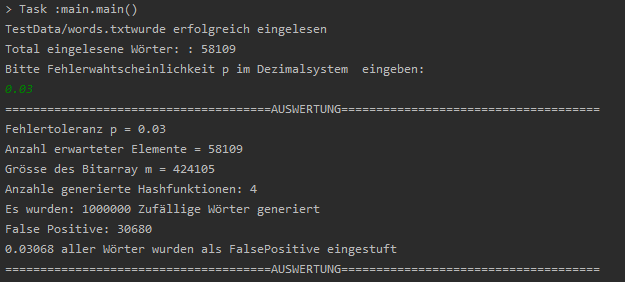
\includegraphics[width=0.7\textwidth]{Ausgabe_Java.png}
\subsubsection{Quellen}
https://www.youtube.com/watch?v=bEmBh1HtYrw
\\ https://de.wikipedia.org/wiki/Bloomfilter
\end{document}